\section{Implementation}

As your spectrum analyzer works on a block of samples 
at a time, you will need to use interrupts to pause 
your processing while samples are transferred from/to 
the CODEC (A/D and D/A) buffer.  
Fortunately, the interrupt handling routines have been 
written for you in a C shell program available 
at \verb+v:\ece320\54x\dspclib\lab4main.c+ and the 
core code.

\subsection{Interrupt Basics}

Interrupts are an essential part of the operation of 
any microprocessor.  They are particularly important in 
embedded applications where DSPs are often used.  
Hardware interrupts provide a way for interacting with 
external devices while the processor executes code.  
For example, in a key entry system, a key press would 
generate a hardware interrupt.  The system code would then 
jump to a specified location in program memory where a 
routine could process the key input.  Interrupts provide 
an alternative to polling.  Instead of checking for 
key presses at a predetermined rate (requires 
a clock), the system could be busy executing other code.  
On the TI-C54x DSP, interrupts provide a convenient way to
transfer blocks of data to/from the CODEC in a 
timely fashion.

\subsection{Interrupt Handling}

The \verb+lab4main.c+ and the core code are intended to 
make your interaction with the hardware much simpler.  
At the heart of this interaction is the auto-buffering 
serial port.  In the auto-buffering serial mode, the 
TI-C54x processor is able to do processing 
{\bf uninterrupted} while samples are transferred to/from a
buffer of length \verb+BlockLen+=$64$ samples.  
However, the spectrum analyzer to be implemented 
in this lab works over a block of $N=1024$ samples.  
If it were possible to compute a $1024$-point FFT 
in the sample time of one \verb+BlockLen+, then no 
additional interrupt handling routines would be 
necessary.  Samples could be collected in a $1024$-length 
buffer and a $1024$-point FFT could be computed 
uninterrupted while the auto-buffering buffer fills.  
Unfortunately, the DSP is not fast enough to 
accomplish this task.

We now provide an explanation of the shell C program 
\verb+lab4main.c+ listed in Appendix A.  The 
\verb+lab4main.c+ file contains the function 
\verb+interrupt void irq+ and a main program.  The main 
program is an infinite loop over blocks of $N=1024$ 
samples.  Note that while the DSP is executing instructions in
this loop, interrupts occur every \verb+BlockLen+ samples.  
Inside the infinite loop, you will insert 
code to do the operations which follow. 
Although each of these operations may be performed in C or 
assembly, we suggest you follow the guidelines suggested.
\begin{enumerate}
   \item{Transfer inputs and outputs (C)}
   \item{Apply a Hamming Window (C/assembly)}
   \item{Bit-reverse the input (assembly)}
   \item{Apply an $N$-point FFT (assembly)}
   \item{Compute the magnitude-squared spectrum (C/assembly)}
   \item{Include a trigger pulse (C/assembly)}
\end{enumerate}

An interrupt from the CODEC occurs every \verb+BlockLen+ samples.  The 
\verb+SetAudioInterrupt(irq)+ call in the main program tells 
the core code to jump to the \verb+irq+ function when an 
interrupt occurs.  In the \verb+irq+ function, \verb+BlockLen+ 
samples of the A/D input in \verb+Rcvptr+ (channel 1) are written 
to a length $N$ \verb+inputs+ buffer, and \verb+BlockLen+ of the 
output samples in the \verb+outputs+ buffer are written to 
the D/A output via \verb+Xmitptr+ on channel 2.  On channel 1 
of the output, the input is echoed out.  {\bf You are to fill 
the buffer \verb+outputs+ with the windowed magnitude-squared 
FFT values by performing the operations listed above.}

In the main code, the \verb+while(!input_full);+ loop waits for 
$N$ samples to collect in the \verb+inputs+ buffer.  Next, 
the $N$ inputs and outputs must be transferred.  You are to 
write this portion of code.  This portion of code is to be done 
first, within \verb+BlockLen+ sample times; otherwise the first 
\verb+BlockLen+ of samples of output would not be available 
on time.  Once this loop is finished, the lengthy processing of the 
FFT can continue.  During this processing, the DSP is interrupted 
every \verb+BlockLen+ samples to transfer samples.  Once this 
processing is over, the infinite loop returns to 
\verb+while(!input_full);+ to wait for $N$ samples to finish 
collecting.

The flow diagram in Figure~\ref{fig:flow} summarizes the operation 
of the interrupt handling routine 
\begin{figure}[ht]
   \begin{center}
      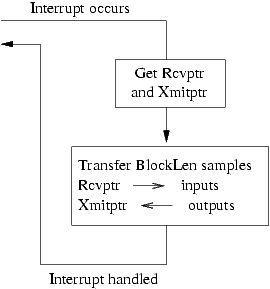
\epsfig{file=interrupt_flow.eps,width=10cm}
      \caption{Flow Diagram of Interrupt Handling.}
      \label{fig:flow}
   \end{center}
\end{figure}

\subsection{FFT Routine}

As the list of operations indicates, bit-reversal and FFT 
computation are to be done in assembly.  
We are providing you with a shell assembly file, 
available at \verb+v:\ece320\54x\dspclib\c_fft_given.asm+ and 
shown in Appendix B, containing many useful declarations and some code.  
The code for performing 
bit-reversal and other declarations needed for the FFT routine are 
also provided in this section.  {\bf However, we would like you 
to enter this code manually, as you will be expected to 
understand its operation.}  

Now, we explain how to use the FFT routine provided by 
TI for the C54x.
The FFT routine \verb+fft.asm+ located in
\verb+v:\ece320\54x\dsplib\+ computes an in-place, complex FFT.
The length of the FFT is defined as a label  
\verb+K_FFT_SIZE+ and the algorithm assumes that the
input starts at data memory location \verb+_fft_data+.
To have your code assemble for an $N$-point FFT, you will have to
include the following label definitions in your assembly code.
\begin{verbatim}
N                 .set       1024
K_FFT_SIZE        .set       N           ; size of FFT
K_LOGN            .set       10          ; number of stages (log_2(N))
\end{verbatim}
In addition to defining these constants, you will have to
include twiddle-factor tables for the FFT.  These
tables (\verb+twiddle1+ and \verb+twiddle2+) are 
available in the shared directory \verb+v:\ece320\54x\dsplib\+.
Note that the tables are each $N$ points long representing values
from $0$ to just shy of $180$ degrees and must
be accessed using a {\bf circular pointer}. To include these
tables at the proper location in memory with the appropriate
labels referenced by the FFT, use the following
\begin{verbatim}
             .sect  ".data"
             .align  1024
sine         .copy "v:\ece320\54x\dsplib\twiddle1"
             .align  1024
cosine       .copy "v:\ece320\54x\dsplib\twiddle2"
\end{verbatim}

%AUTHOR: Michael Kramer
The FFT provided requires that the input be in bit-reversed
order, with alternating real and imaginary components.
Bit-reversed
addressing is a convenient way to order input $x[n]$
into a FFT so that the output $X(k)$ is in sequential order
(i.e. $X(0), X(1),\ldots X(N-1)$ for an $N$-point FFT).
The following table illustrates the bit-reversed order for
an eight-point sequence.
\begin{center}
\begin{tabular}{|c|c|c|c|} \hline
Input Order & Binary Representation & Bit-Reversed Representation
& Output Order \\ \hline
0 & 000 & 000 & 0 \\
1 & 001 & 100 & 4 \\
2 & 010 & 010 & 2 \\
3 & 011 & 110 & 6 \\
4 & 100 & 001 & 1 \\
5 & 101 & 101 & 5 \\
6 & 110 & 011 & 3 \\
7 & 111 & 111 & 7 \\
\hline
\end{tabular}
\end{center}

The following routine performs the bit-reversed
reordering of the input data.  
The routine assumes that the input is stored in data memory
starting at the location labeled \verb+_bit_rev_data+, which must 
be aligned to the least power of two greater than the input buffer 
length, and consists of 
alternating real and imaginary parts.  
Because our input data is going to be purely real in this
lab, you will have to make sure that you set the imaginary
parts to zero by zeroing out every other memory location.

\setlength{\baselineskip}{0.39cm}
\setlength{\parskip}{0.4cm}
\listinginput{1}{bit_rev.asm}
\setlength{\baselineskip}{0.5cm}
\setlength{\parskip}{0.5cm}

As mentioned, in the above code \verb+_bit_rev_data+ is a label indicating
the start of the input data and \verb+_fft_data+ is a label indicating 
the start of a circular buffer where the bit-reversed data will be written.
Note that although \verb+AR7+ is not
used by the bit-reversed routine directly, it is used extensively
in the FFT routine to keep track of the start of the FFT data space.

In general, to have a pointer index memory in bit-reversed order, the
\verb+AR0+ register needs to be set to one-half the length of
the circular buffer; a statement such as \verb!ARx+0B! is
used to move the \verb+ARx+ pointer to the next location.
For more information regarding the bit-reversed
addressing mode, refer to page 5-18 in the {\em TI-54x CPU and Peripherals}
manual.  Is it possible to bit-reverse a buffer in place?  For 
a diagram of the ordering of the data expected by the FFT routine, 
see Figure 4-10 in the {\em TI-54x Applications Guide}.  Note that the 
FFT code uses all the pointers available and does not 
restore the pointers to their original values.





\subsection{Creating the Window}
As mentioned, you will be using the FFT to compute the spectrum
of a windowed input.  For your implementation you will need 
to create a 1024-point Hamming window.  
Create a Hamming window in \matlab using the function 
\verb+hamming+, then use \verb+save_coef+ to save the window
to a file that can then be included in your code with
the \verb+.copy+ directive.

\subsection{Displaying the Spectrum}

Once the DFT has been computed, you must calculate the
squared magnitude of the spectrum for display.
\bea
| X(k) | ^2 & = & \mbox{Re}\;\{ X(k) \} ^2 + \mbox{Im} \;\{ X(k) \} ^2
\label{equ:squared magnitude}
\eea
You may find the assembly instructions \verb+squr+ and \verb+squra+
useful in implementing (~\ref{equ:squared magnitude}).

Because the squared magnitude is always nonnegative, you can
replace one of the magnitude values with a $-1.0$ as a trigger pulse
for display on the oscilloscope.
This is easily performed by replacing the DC term ($k=0$) with
a $-1.0$ when copying the magnitude values to the output buffer.
The trigger pulse is necessary for the oscilloscope to
lock to a specific point in the spectrum and keep the
spectrum fixed on the scope.

\subsection{Intrinsics}
If you are planning on writing some of the code in C, then you 
may be forced to use intrinsics.  Intrinsic instructions provide a 
way to use assembly instructions directly in C.  An example of an 
intrinsic instruction is 
\verb+bit_rev_data[0]=_smpyr(bit_rev_data[0],window[0])+ which 
performs the assembly signed multiply round instruction.  You may also 
find the \verb+_lsmpy+ instruction useful.  For more information on 
intrinsics, see page 6-22 of the {\em TI-C54x Optimizing C/C++ Compiler 
User's Guide} available on the course web page.

\section{Quiz Information}
From your prelab experiments, you should be able to describe the 
effect of windowing and zero-padding on FFT spectral analysis.  
In your DSP system, experiment with different inputs, 
changing $N$ and the type of window.  Does the $|X(k)|^2$ coincide 
with what you expect from \matlab?  What is the relationship 
between the observed spectrum and the DTFT.

\newpage
\section{Appendix A:}
\setlength{\baselineskip}{0.39cm}
\setlength{\parskip}{0.4cm}
\listinginput{1}{./code/lab4main.c}
\setlength{\baselineskip}{0.5cm}
\setlength{\parskip}{0.5cm}

\newpage
\section{Appendix B:}
\setlength{\baselineskip}{0.39cm}
\setlength{\parskip}{0.4cm}
\listinginput{1}{./code/c_fft_given.asm}
\setlength{\baselineskip}{0.5cm}
\setlength{\parskip}{0.5cm}

\end{document}
\bye



